\documentclass{beamer}
\usepackage[utf8]{inputenc}
\title{TkDQMDoctor}
\subtitle{Certification Helper}
\author{\texorpdfstring{Filip Ilic\newline\url{filip.ilic@cern.ch}}{Filip ilic}}
\date{\today}

\begin{document}
\maketitle


\begin{frame}
  \frametitle{Motivation} 
  Management system to create shift reports, and keep track of known issues. 
	\begin{itemize}
	\item Problems that have been solved might be forgotten after a while and need to be solved again. 
	\item Solution: Create a centralized system that keeps track of issues and their solutions. 
Ultimately a system that can give guidance to shifters while taking known issues into consideration is envisioned.
	\item Similar system successfully used: DAQDoctor
	\end{itemize}
\end{frame}


\begin{frame}
\frametitle{TkDQMDoctor - Overview}
  \begin{columns}[T]
    \begin{column}{.5\textwidth}
     \begin{block}{}

\begin{itemize}
\item Certification Helper
\begin{itemize}
	\item Input forms during run certification.
\end{itemize}
\item Doctor
\begin{itemize}
	\item Interfaces with the Certification Helper and Database of known Issues.
\end{itemize}
\item Database of known Issues
\end{itemize}

   	\end{block}	
    \end{column}
    \begin{column}{.5\textwidth}
    \begin{block}{}
    \begin{figure}[h]
    \phantom{g}
	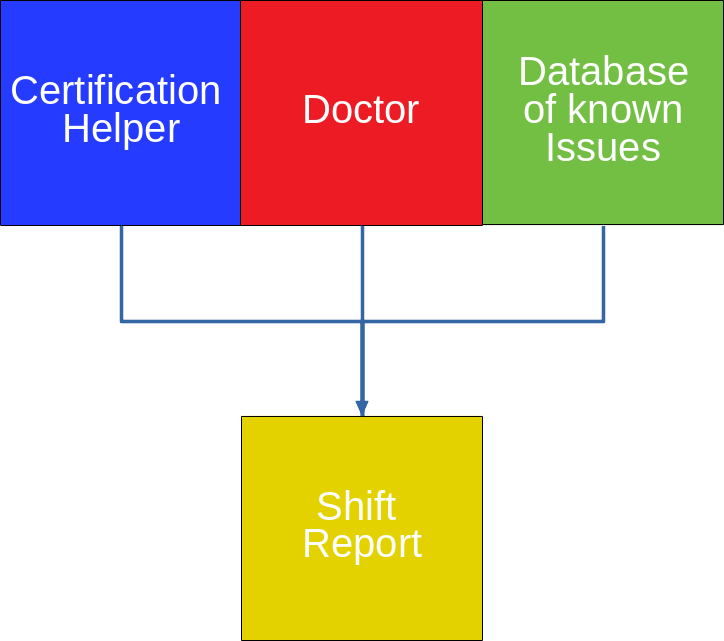
\includegraphics[width=0.7\textwidth]{figures/overview.png}
			\end{figure}

    \end{block}
    \end{column}
  \end{columns}
\end{frame}


\begin{frame}
\frametitle{Certification Helper}
  \begin{columns}[T]
   \begin{column}{.5\textwidth}
   \begin{block}{}

\begin{itemize}
 \item Overall Goal: Help shifters create good reports
 \item Checklist pages for each quality flag
 \item Guiding to the corresponding Twiki pages
 \item Produce \textbf{automated} shift report
\end{itemize}
   	\end{block}	
    \end{column}
    \begin{column}{.5\textwidth}
    \begin{block}{}
        \begin{figure}[h]
        \phantom{g}
		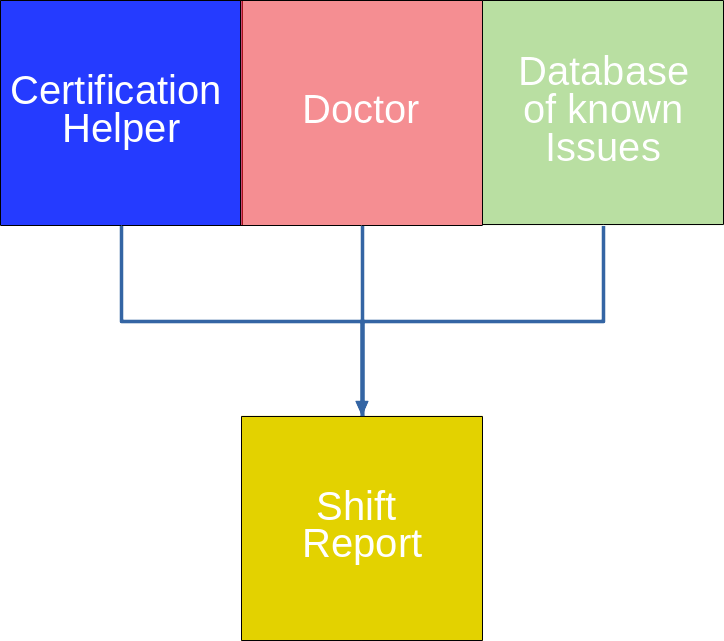
\includegraphics[width=0.7\textwidth]{figures/overview_1.png}
		\end{figure}
    \end{block}
    \end{column}
  \end{columns}
\end{frame}

\begin{frame}
  \frametitle{Current state}
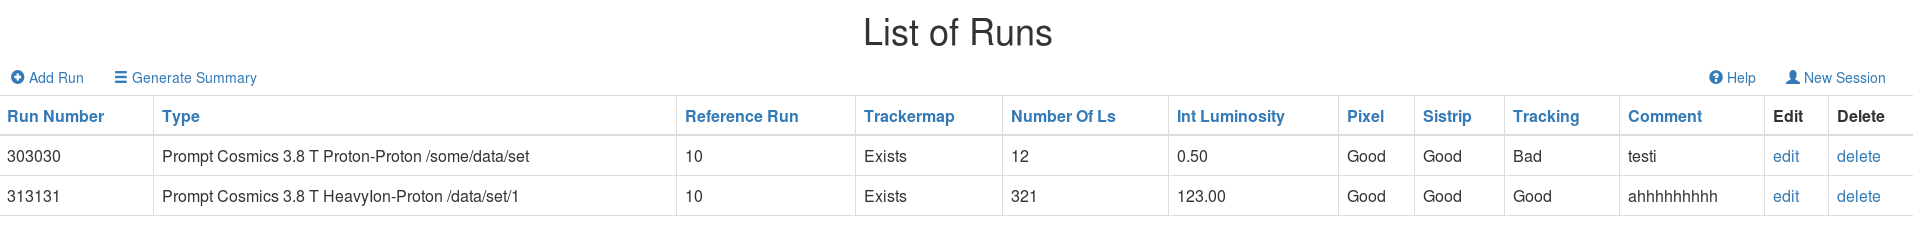
\includegraphics[width=\textwidth]{figures/list.png}\\
Current web interface.\\
\begin{itemize}
\item List of runs that were added in this session.
\item All the usual stuff possible: sorting, editing, deleting
\item Generating shift report from the runs in this session
\end{itemize}
\end{frame}

\begin{frame}
  \frametitle{Certifying a run}
  \begin{columns}[T]
    \begin{column}{.5\textwidth}
    \begin{block}{}

	Adding a new run works through this form
	\begin{itemize}
	\item Mostly dropdown menus (reducing errors)
	\item Next to each field a link to a checklist page, detailing the procedure for checking that quality flag. (guiding)
	\end{itemize}
   	\end{block}	
    \end{column}
    \begin{column}{.5\textwidth}
    \begin{block}{}
	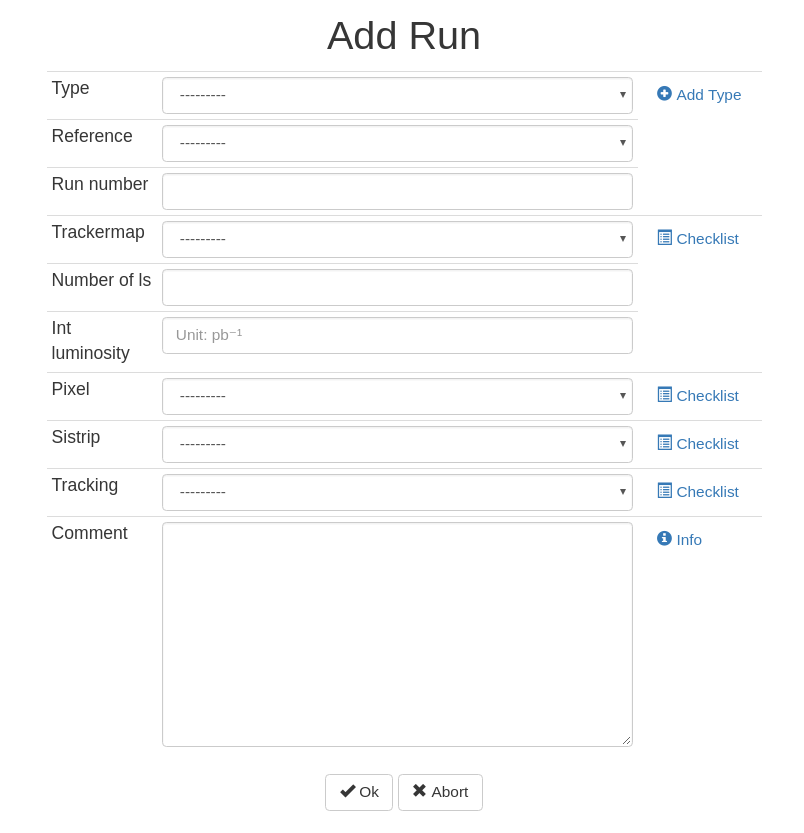
\includegraphics[width=\textwidth]{figures/add_run.png}
    \end{block}
  \end{column}
\end{columns}
\end{frame}

\begin{frame}
\frametitle{Certifying a run - Error Messages}
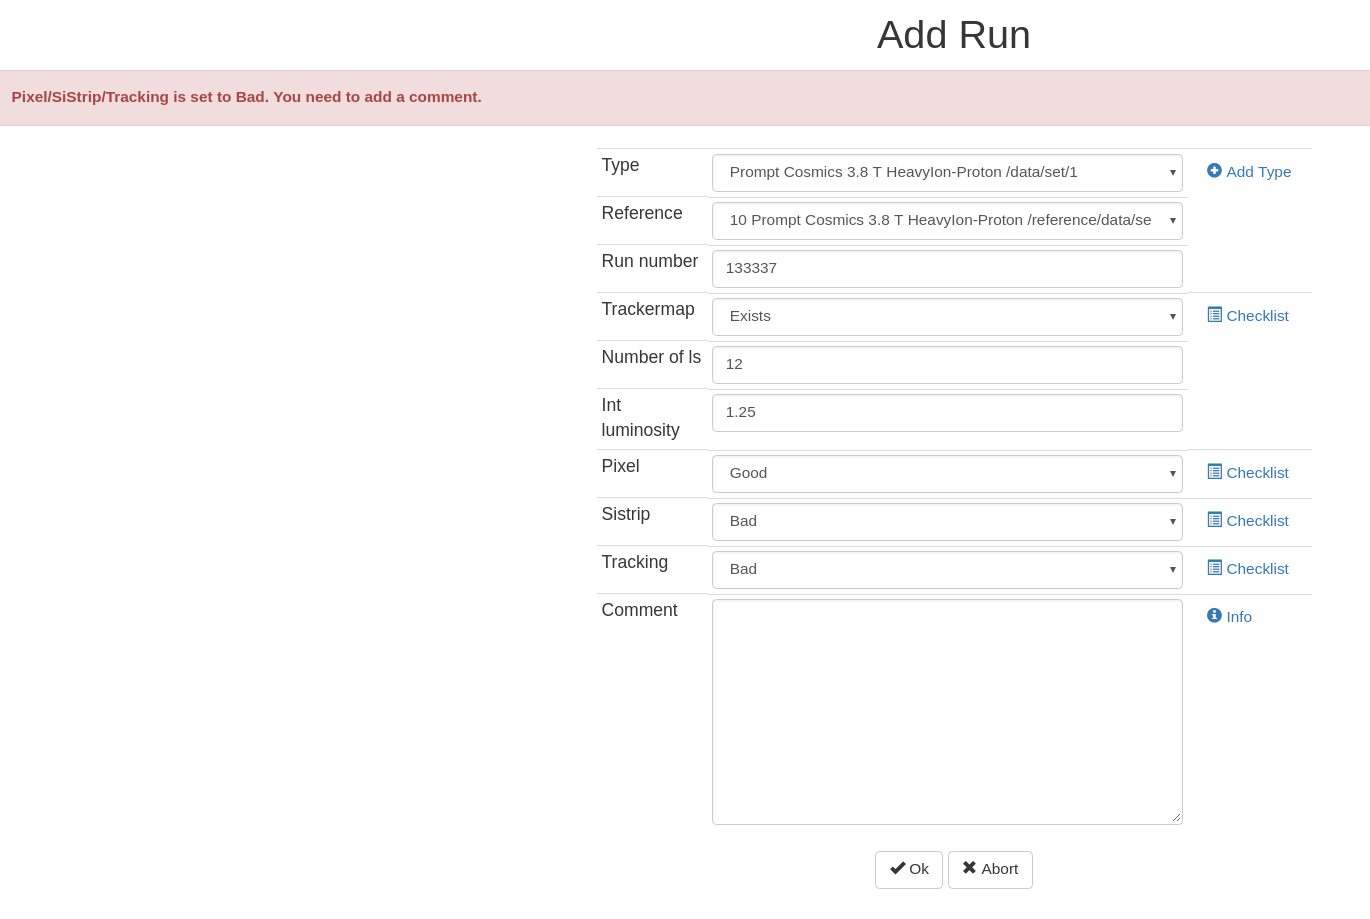
\includegraphics[width=\textwidth]{figures/error.png}\\
Correctness checks: Pixel/Strip/Tracking are set to 'Bad' while there is no comment giving additional information.
\end{frame}


\begin{frame}
  \frametitle{Adding a run type}
  \begin{columns}[T]
    \begin{column}{.5\textwidth}
    \begin{block}{}

	Adding a new run type works again through a dialog
	\begin{itemize}
	\item Mostly dropdown menus
	\end{itemize}
   	\end{block}	
    \end{column}
    \begin{column}{.5\textwidth}
    \begin{block}{}
	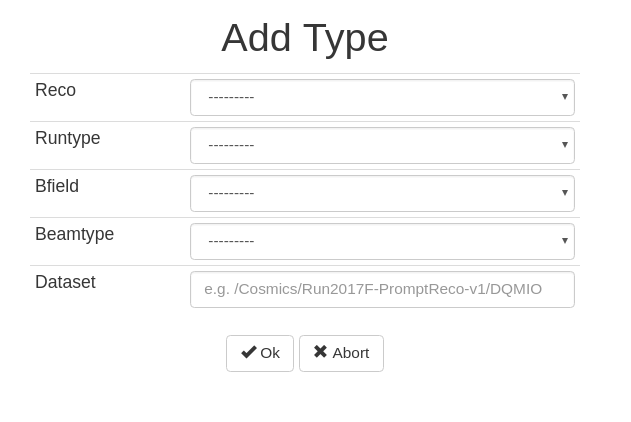
\includegraphics[width=\textwidth]{figures/add_type.png}
    \end{block}
  \end{column}
\end{columns}
\end{frame}

\begin{frame}
  \frametitle{Adding a reference run}
  \begin{center}
  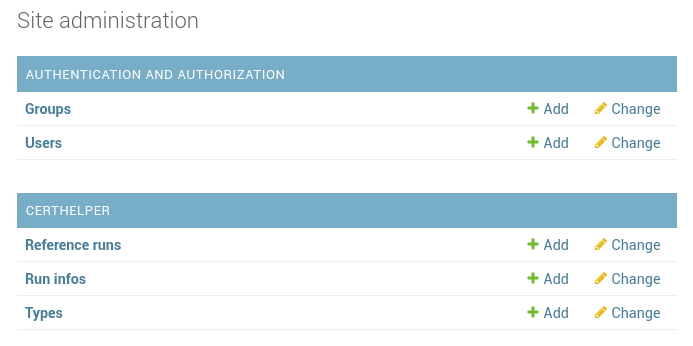
\includegraphics[width=0.4\textwidth]{figures/admin_1.png}
  \end{center}
  \begin{columns}[T]
    \begin{column}{.5\textwidth}
    \begin{block}{}
	\begin{itemize}
	\item Can not be done by shifters.
	\item Currently only possible through the admin page.
	\end{itemize}
   	\end{block}	
    \end{column}
    \begin{column}{.5\textwidth}
    \begin{block}{}
		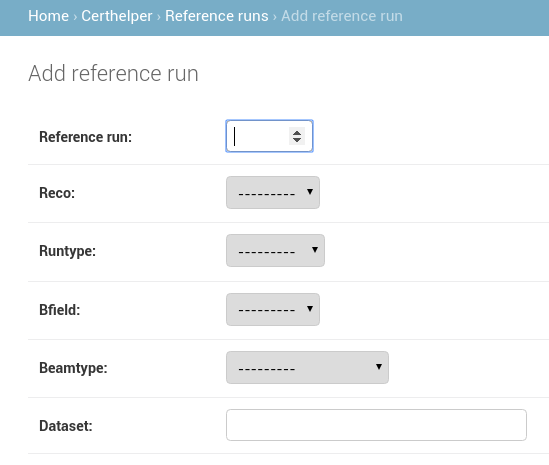
\includegraphics[width=\textwidth]{figures/admin_2.png}
    \end{block}
  \end{column}
\end{columns}
\end{frame}

\begin{frame}
  \frametitle{Report Summary}
  \begin{columns}[T]
    \begin{column}{.5\textwidth}
    \begin{block}{}
	\begin{itemize}
	\item Summary is auto generated based on the runs in the current session.
	\item What goes in the \textbf{HDQM Trends} section?
	\end{itemize}
   	\end{block}	
    \end{column}
    \begin{column}{.5\textwidth}
    \begin{block}{}
	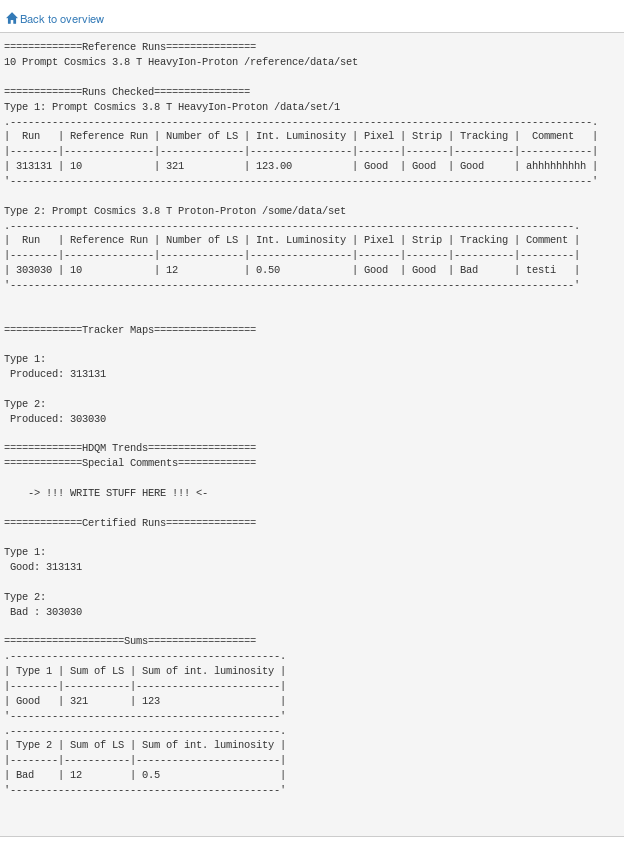
\includegraphics[width=\textwidth]{figures/summary.png}
    \end{block}
  \end{column}
\end{columns}
\end{frame}



\begin{frame}
  \frametitle{Conclusions}
  \begin{itemize}
  \item We think the Certification Helper is mature enough to be used, starting Monday (4.12.2017).
  \item We are hoping to gather some feedback / find bugs.
  \item Currently in the process of deploying it.
  \end{itemize}
\end{frame}

\begin{frame}
  \frametitle{Questions}
  \begin{itemize}
    \item What checks must be performed on the input forms to guarantee validity?\\(e.g. no comment + one of the quality flags is 'Bad')
    \item What belongs in the \textbf{HDQM} section of the shift report? 
  \end{itemize}
\end{frame}


\begin{frame}
\begin{itemize}
\item Repository: https://github.com/imKuehlschrank/TkDQMDoctor
\item Suggestions/Feedback: filip.ilic@cern.ch, jandrea@cern.ch
\end{itemize}
\end{frame}

\end{document}